\section{Proposed approach}
\label{sec:approach}

\subsection{Overview}

\subsection{Breaking down the DSLs}

The objective of this step is to divide the DSL in several language modules that can be latter composed. To do so, we need to deal with two problems. The former is to find the way in which the we will split the language constructs. The second one is to define the language modules themselves with their corresponding required and provided interfaces. 

\subsubsection{Identifying constructs distribution}

The input is the set of DSLs. We first identify the language constructs for each one. Then we perform a match according to a given comparison operator. Then, we merge. Finally, we execute a graph partitioning algorithm. 

\begin{figure*}
\centering
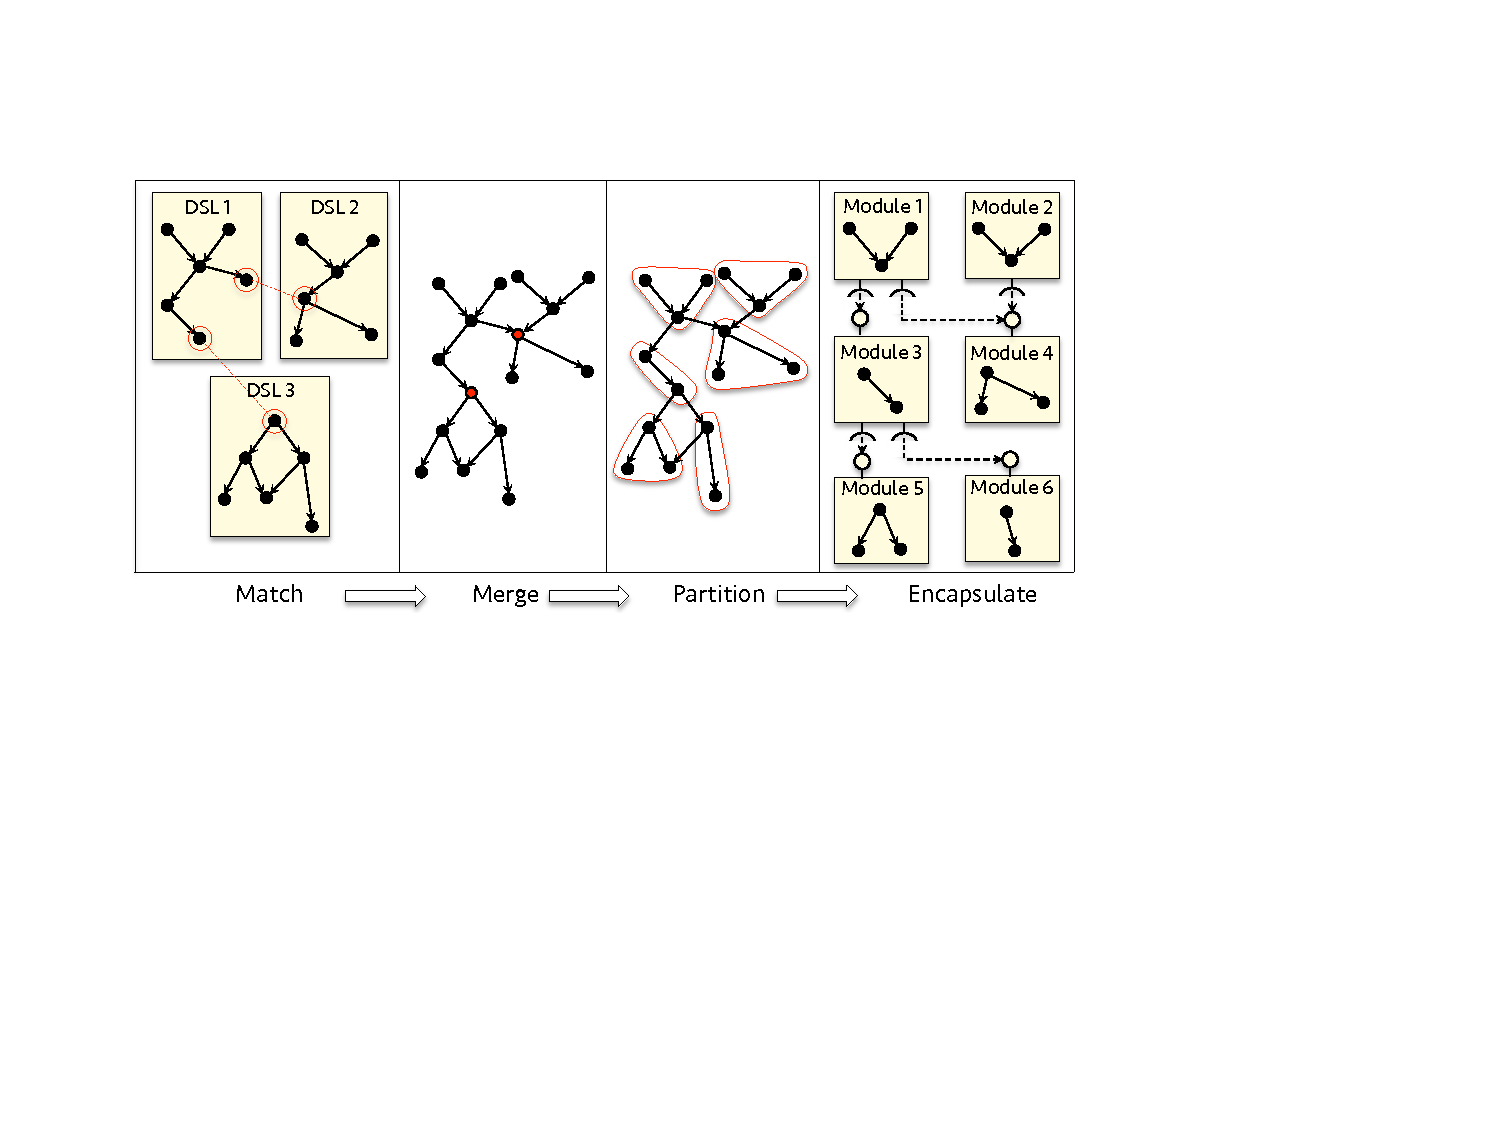
\includegraphics[width=1\linewidth]{images/breaking-down.pdf}
\caption{Process for breaking down a set of DSLs}
\label{fig:breaking-down}
\end{figure*}

\subsubsection{Specifying language modules}

Note that both DSLs and modules are, at the end, set of language constructs. Hence, one may think that a module is also a DSL. Although this is technically true, there is a substantial difference between DSLs and modules. A DSL is a closed set of constructs that materializes a complete DSL specification that is ready to be used. Contrariwise, a module is set of constructs whose specification may depend on other constructs defined in other modules. A module can be used (and considered itself as a DSL) as long as their dependencies are fulfilled.

Accordingly, the main requirement for supporting separation of features in DSLs relies on the capability of expressing dependencies between language modules. In this context, we have identified two types of dependencies: \textit{aggregation} and \textit{extension}. In the following, we explain each of them and we present the corresponding tool support.

\textbf{Language modules \textit{aggregation}:} In aggregation, there is a \textit{requiring module} that \underline{uses} some constructs provided by a \textit{providing module}. The requiring module has a dependency relationship towards the providing one that, in the small, is materialized by the fact that some of the classes of the requiring module have references (simple references or containment references) to some constructs of the providing one.

In order to avoid direct references between modules, we introduce the notion of interfaces for dealing with modules' dependencies. In the case of aggregation, the requiring language has a \textit{required interface} whereas the providing one has the \textit{provided interface}. A required interface contains the set of constructs required by the requiring module which are supposed to be replaced by actual construct provided by other module(s).

It is important to highlight that we use \textit{model types} \cite{Steel:2007} to express both required and provided interfaces. As illustrated on top of Figure \ref{fig:approaches-interfaces}, the relationship between a module and its required interface is \textit{referencing}. A module can have some references to the constructs declared in its required interface. In turn, the relationship between a module and its provided interface is \textit{implements} (deeply explained in \cite{Degueule:2015}). A module implements the functionality exposed in its model type. If the required interface is a subtype of the provided interface, then the provided interface fulfills the requirements declared in a required interface. Note that the partial sub-typing relationship defined in \cite{Guy:2012}, permits a required interface being partially fulfilled by a provided interface. The result of the composition will be a module with a new required interface that contains only those elements that were not provided.


\textbf{Language modules \textit{extension}:} In this case, there is an extension module that (naturally) \underline{extends} the functionality provided by \textit{base module}. The extension module has a dependency to the base module. Moreover, the extension module has little sense by itself without the existence of a base module \cite{Erdweg:2012}. Note that this is a conceptual difference with respect to modules aggregation where the required make sense by itself but requires some external services in order to work correctly.

There are to different mechanisms for extending a base module: \textit{constructs specialization} and \textit{open classes} \cite{Clifton:2000}. In constructs specialization, the constructs of the base module can be extended by adding new subclasses. The extension module contains the new subclasses that reference (by means of the inheritance relationship) the constructs of the base module that are being extended. In this case, the base module remains intact in after the composition but there are additional constructs. In open classes, constructs of the base module can be re-opened and modified by the extension module. For example, for adding a new attribute to a given construct without creating a sub-class, or for overriding a given segment of the semantics. In this case, the extension module is altered after the composition phase. 

Similarly to aggregation, dependencies between the base and the extension modules are specified through interfaces. The base module exposes an \textit{extension point interface} with the constructs that can be extended. In turn, the \textit{extension interface} declares the constructs of the base module that are being extended.

Like in aggregation, and as illustrated at the bottom of Figure \ref{fig:approaches-interfaces}, we use model types of expressing these interfaces. Although the approach is quite similar, there is one fundamental difference between the interfaces in aggregation and the interfaces in extension: the relationship between an extension module and its extension interface is \textit{usage} more than just referencing. That means that the module can to reference the elements declared in the required interface and also modify them by adding new elements. This capability is introduced to support extension by the open-classes mechanism.

\begin{figure*}
\centering
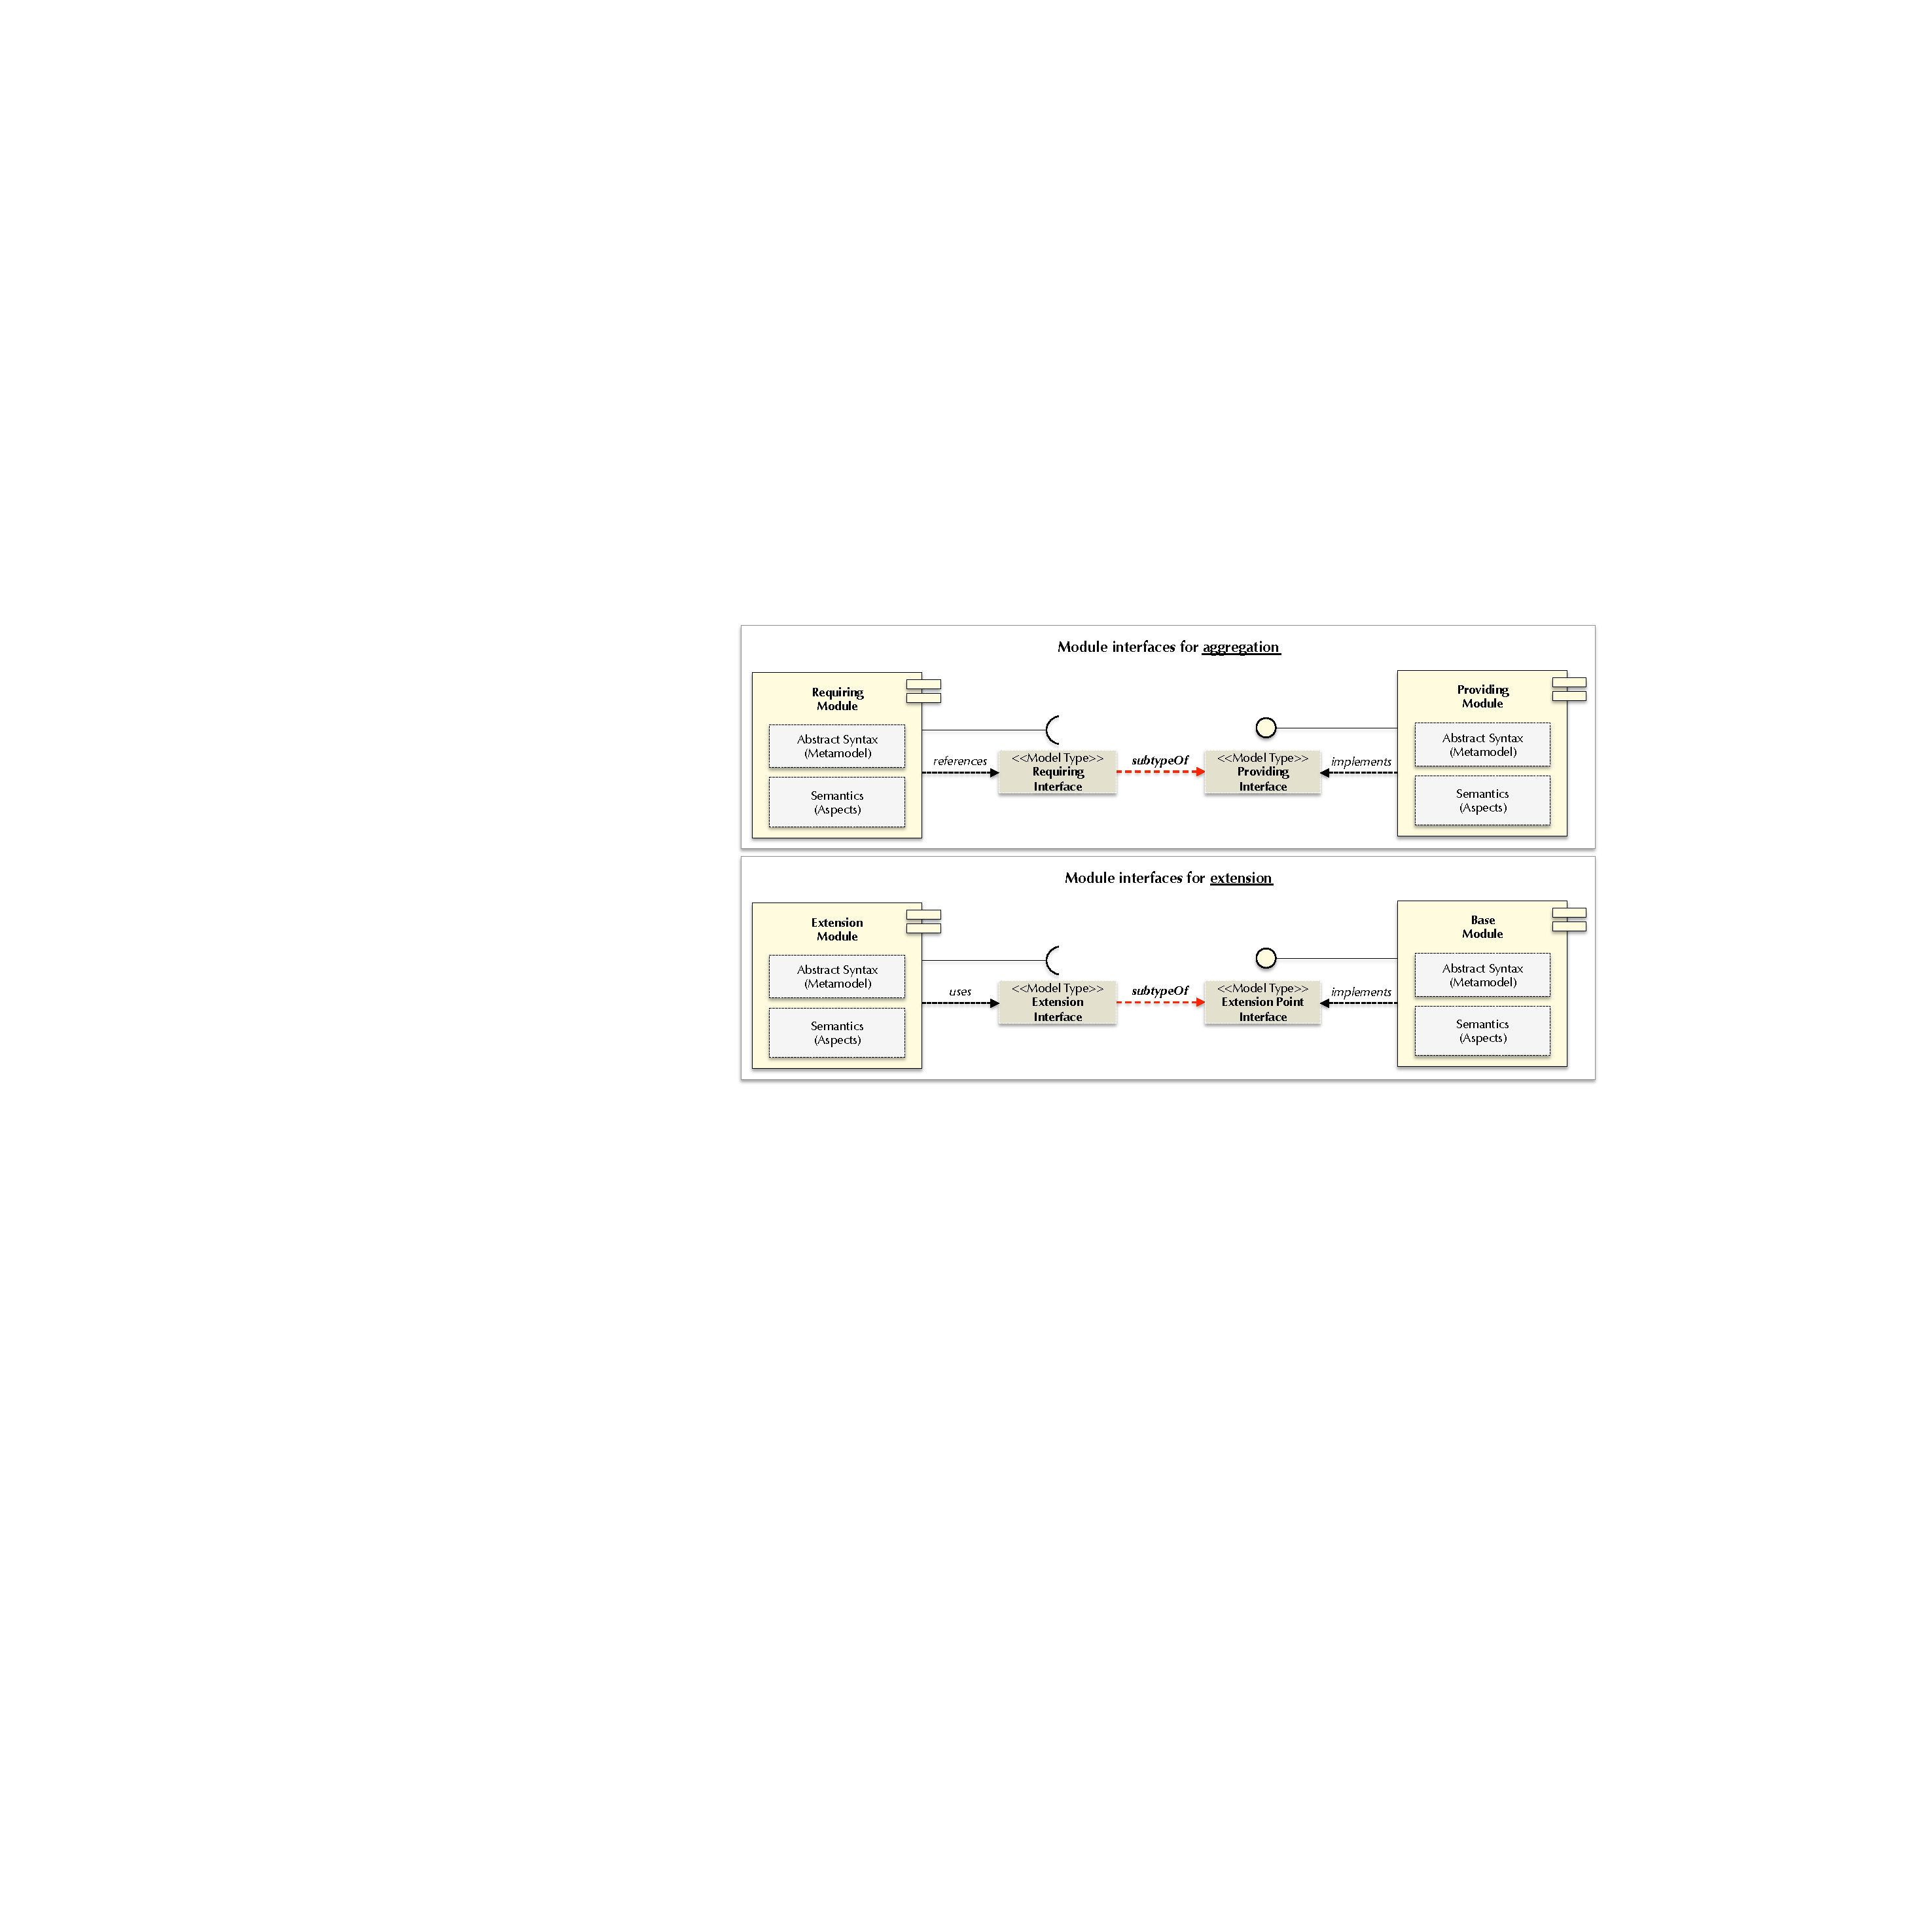
\includegraphics[width=1\linewidth]{images/approaches-interfaces.pdf}
\caption{Interfaces for modularization of DSLs}
\label{fig:approaches-interfaces}
\end{figure*}

\subsection{Inferring the variability model}

After having a set of language modules with their corresponding references among them, we need to automatically infer a variability model that represents the existing variability. To do so, we use as input an algorithm that, based on the dependencies graph of the modules, infer a simple variability model. 



\subsection{Deriving a DSL}

Once the variability of the language product line is correctly specified, the next step is to configure DSLs by using the variability model. Since the variability model is expressed in CVL, the configuration of the language product corresponds to the specification of a realization model that captures the decisions made by the language designers that are configuring the DSL. Our approach uses the realization model to produce the corresponding Melange script. 

As an example, consider the configuration presented in the variability model of the Figure \ref{fig:multi-dimensional-variability}. The corresponding Melange script is presented in the following listing code snippet:

\begin{lstlisting}
language ModuleA {
   ecore MetamodelA.ecore
   with package.A.Semantics6
}

language ModuleB {
   ecore MetamodelB.ecore
   with package.B.Semantics4
}

language MyDSL {
   aggregation(ModuleB, ModuleA)
}
\end{lstlisting}

Note that the Melange script only contains the language elements that correspond to a given configuration. For example, the ModuleA contains only the Semantics6 because it was the choice made at configuration time. Similarly, ModuleB only contains Semantics4. Note also that there is a third language appearing in the script: MyDSL. This language represents the composition of the language modules and can be understood as the root of the script. In this case, this statement of Melange indicates that the modules A and B are composed by aggregation. The first element in the operation corresponds to the requiring module and the second element corresponds to the providing module. 

Once the configuration process produces a Melange script that captures the choices made by the language designers for a particular DSL, it is necessary to compose the declared language modules and produce the DSL. The composition of a set of modules requires a previous phase of compatibility checking. Not all language modules are compatible and in that case composition cannot be performed. In our approach, check the compatibility of two language modules is to verify the sub-typing relationship between the required and provided interface (for the case of aggregation), and the extension and extension point interfaces (for the case of extension).

Once this compatibility checking is correctly verified, language modules are composed. In particular, their specifications are be merged to generate a complete language specification. This merging basically replaces the elements of the required interface by its corresponding implementation in the provided component. A similar process is performed in the case of extension. 